%&latex
%
\documentclass[../template.tex]{subfiles}
\usepackage{graphicx}

\begin{document}

%\section{Microcanonical - part 2}
We now substitute (\ref{eqn:heav-deriv}) and (\ref{eqn:z-omega}) in (\ref{eqn:pQP}), leading to:
\begin{align}\label{eqn:pQP1}
    P(\mathbb{Q}, \mathbb{P}) = \frac{1}{\mathcal{Z}} \delta \mathcal{E}\cdot \delta (\mathcal{E}- H(\mathbb{Q}, \mathbb{P})) \underset{\delta \mathcal{E} \to 0}{=} \frac{\delta(\mathcal{E}-H(\mathbb{Q}, \mathbb{P}))}{\Omega(\mathcal{E}, V, N)} 
\end{align}

Then, we can compute the (microcanonical) average for any given observable $O(\mathbb{Q},\mathbb{P})$ as follows:
\begin{align*}
    \langle O \rangle = \int_{\mathbb{R}^{6N}} \dd{\bm{\Gamma}} \mathbb{P}(\mathbb{Q}, \mathbb{P}) O(\mathbb{Q}, \mathbb{P}) \underset{\delta \mathcal{E} \to 0}{=} \frac{1}{\Omega} \int_{\mathbb{R}^{6N}} \dd{\bm{\Gamma}} \delta(\mathcal{E}- H(\mathbb{Q},\mathbb{P})) O(\mathbb{Q},\mathbb{P})
\end{align*}

\subsection{Ideal gas}
Now that we have obtained the microcanonical distribution, we can use it to compute thermodynamic quantities, such as energy, temperature, pressure.

\medskip

To make explicit calculations we need to fix the \textit{specifics} of the system we are working with, and in particular its \textbf{Hamiltonian} (\ref{eqn:hamiltonian}). 

So, we start by considering the simplest possible case, where there are \textit{no interactions} between the $N$ particles, meaning that:
\begin{align} \label{eqn:no-interaction}
    U_{\mathrm{int}}(\mathbb{Q}) = 0
\end{align} 
Thus the Hamiltonian involves only \textit{translational} kinetic energies:
\begin{align}\label{eqn:h-ideal-gas}
    H(\mathbb{Q},\mathbb{P}) = \sum_{i=1}^N \frac{\norm{\bm{p_i}}^2}{2m} = \frac{\norm{\mathbb{P}}^2}{2m} \equiv H(\mathbb{P})
\end{align}
This is the key hypothesis of the (monoatomic\footnote{If we consider molecules we need also to account the \textit{rotational kinetic energies}.}) \textbf{ideal gas} model, which approximates the behaviour of real gases at sufficiently high temperature and low pressure.

\medskip

However, \textit{some amount of interaction} needs to be present if we want the gas to reach equilibrium. Otherwise,  the $\norm{\bm{p}_i}$ of each particle $i$ would be conserved, meaning that the velocity distribution would remain always that of the initial state. So, more precisely, we consider:
\begin{align*}
    0 \neq U(\mathbb{Q}) \ll |\mathcal{E}|
\end{align*}  
In this way we can study equilibrium and still neglect $U_{\mathrm{int}}$ in our calculations, as the kinetic energy always \textit{prevails}. 

\medskip

Note that $H$ in (\ref{eqn:h-ideal-gas}) depends only on $\mathbb{P}$, and so also the probability density of \textit{configurations}, which can be obtained by \textit{marginalizing} the joint pdf $\mathcal{P}(\mathbb{Q},\mathbb{P})$ over $\mathbb{P}$, must be independent of $\mathbb{Q}$ - and so it must be uniform over the \q{allowed} domain $V_N$:
\begin{align}\label{eqn:pQ1}
    P(\mathbb{Q}) = \int_{\mathbb{R}^{3N}} \dd[3N]{\mathbb{P}} \mathcal{P}(\mathbb{Q},\mathbb{P}) = \frac{1}{\Omega} \int_{\mathbb{R}^{3N}} \dd[3N]{\mathbb{P}} \delta\left(\mathcal{E}- \frac{\norm{\mathbb{P}}^2}{2m} \right) = \frac{1}{A} \bb{1}_{V_N}(\mathbb{Q})
\end{align}
Here $V_N$ is the subset of $\mathbb{Q}$ containing the \textit{possible} configurations, which are constrained to have a \textbf{fixed volume}:
\begin{align*}
    V_N = \{Q_N \in \mathbb{R}^{3N} \colon (x_i, y_i, z_i) \in V, \> i = 1, \dots, N\}
\end{align*} 
And $A$ is the normalization factor, given by:
\begin{align}
    A = \int_{V_N} \dd[3N]{\mathbb{Q}} = \int_{V_N} \prod_{i=1}^{N} \dd{x_i}\dd{y_i}\dd{z_i} = \prod_{i=1}^N \underbrace{\int_V \dd{x}\dd{y}\dd{z}}_{V}  = V^N
\end{align}

Substituting in (\ref{eqn:pQ1}) we arrive to:
\begin{align} \label{eqn:pQ2}
    \mathbb{P}(\mathbb{Q}) = \frac{1}{V^N} \bb{1}_{V_N}(\mathbb{Q}) = \begin{cases}
        \frac{1}{V^N} & \bm{r_i} \in V \> \forall i\\
        0 & \text{otherwise} 
    \end{cases} 
\end{align}

In the definition of $\Omega$ (\ref{eqn:omega-def}) we can then integrate over the $\mathbb{Q}$, which just leads to a factor of $V^N$, leading to: 
\begin{align}\nonumber
    \Omega(\mathcal{E}, V, N) &= \int_{\mathbb{R}^{6N}} \dd{\bm{\Gamma}} \delta\left(\mathcal{E}-\frac{\norm{\mathbb{P}}^2}{2m} \right) = \underbrace{\int_{V_N} \dd{\mathbb{Q}}}_{V^N} \underbrace{\int_{\mathbb{R}^{3N}} \dd{\mathbb{P}} \delta\left(\mathcal{E}- \frac{\norm{\mathbb{P}}^2}{2m} \right) }_{\Omega_1(\mathcal{E},N)}=\\
    & \equiv V^N \Omega_1(\mathcal{E}, N) \label{eqn:omega1-def}
\end{align}

\begin{appr}\textbf{Fixed volume constraint}. The constraint on the volume $V$ is part of the \textit{specification} of the system. In fact, more precisely, it appears as part of the potential term $U(\mathbb{Q})$ in $H$, describing the interaction between the gas particles and the walls.

Explicitly, we can write $U(\mathbb{Q})$ as a sum of two terms:
\begin{align*}
    U(\mathbb{Q}) = U_{\mathrm{int}}(\mathbb{Q}) + \sum_{i=1}^N u(\bm{r_i})
\end{align*}
Here $U_{\mathrm{int}}(\mathbb{Q})$ describes the \textit{particle-particle} interactions, and is such that $0 \neq |U_{\mathrm{int}}(\mathbb{Q})| \ll \mathcal{E}$ as we have seen above. The second term, on the other hand, represents the \textit{particle-wall} interactions. In particular, $u(\bm{r})$ is a \textbf{confining potential}:   
\begin{align*}
    u(\bm{r}) = \begin{cases}
        0 & \bm{r} \in V\\
        +\infty & \bm{r}\not\in V
    \end{cases}
\end{align*}
So, all configurations with at least a particle $\notin V$ are assigned a \textit{infinite} energy $H$, meaning that: 
\begin{align*}
    \delta(\mathcal{E}- H(\mathbb{Q},\mathbb{P})) = \delta\left(\mathcal{E}-\frac{\mathbb{P}^2}{2m} - U(\mathbb{Q}) \right) \underset{|U_{\mathrm{int} }| \ll \mathcal{E}}{\approx}  \delta\left(\mathcal{E}- \frac{\mathbb{P}^2}{2m} - \sum_{i=1}^N u(\bm{r_i}) \right) = 0 \quad \forall \mathcal{E}
\end{align*}
as $\mathcal{E}$ is always finite. It follows that the integrand of (\ref{eqn:pQ1}) is \textit{null} outside $V_N$, and \textit{constant} (as it does not depend on $\mathbb{Q}$) on the inside, leading back to:
\begin{align*}
    \mathbb{P}(\mathbb{Q}) = \frac{1}{\Omega} \int_{\mathbb{R}^{3N}} \dd[3N]{\mathbb{P}} \delta\left(\mathcal{E}- \frac{\mathbb{P}^2}{2m} - \sum_{i=1}^N u(\bm{r_i}) \right) = \frac{1}{V^N} \bb{1}_{V_N} (\mathbb{Q}) 
\end{align*}
\end{appr}

\subsubsection{Probability distribution of the number of particles in half the volume} %TO DO: insert figure
Consider the volume $V$ as divided in two halves, $V_L$ and $V_R$. To simplify notation, we \textit{double} the number of particles in the entire system, meaning that now $V$ contains $2N$ particles. We expect that, at any given instant, $V_L$ and $V_R$ will contain roughly $N$ particles - half of the total number - up to some slight fluctuation. 

\medskip

We can \textit{quantify} this argument by using the microcanonical ensemble. 

Consider the probability $P_m$ that, at a given instant at \textbf{equilibrium}, $N+m$ particles are found in $V_R$, with $m > 0$. According to (\ref{eqn:pQ2}), the probability of any configuration $\mathbb{Q}_0$ is the same. This means that configurations are distributed uniformly in $V_{2N}$, and - as all particles are independent - that each particle is uniformly distributed in $V$. So, for any given $i$, $\bm{r_i} \in V_R$ with probability $1/2$, because $V_R = V/2$ by definition. 

Then $P_m$ can be seen as the probability of \textit{tossing} $2N$ coins and obtaining exactly $N+m$ heads, which is given by a binomial distribution:
\begin{align}\label{eqn:m-binomial}
    P_m = {2N \choose N+m} \left(\frac{1}{2} \right)^{N+m} \left(1-\frac{1}{2} \right)^{N-m} = {2N \choose N+m} 2^{-2N} \qquad -N \leq m \leq N 
\end{align}  
 When both $N\pm m$ are $\gg 1$ we can use the Stirling's approximation:
\begin{align}\label{eqn:stirling1}
    \ln n! = n \ln n - n  +\frac{1}{2} \ln (2 \pi n)  + O\left(\frac{1}{n} \right)
\end{align}
to evaluate $\ln P_n$:
\begin{align*}
    \ln P_m &= \ln \frac{2N!}{(2N-N-m)!(N+m)!} 2^{2N} =\\ 
    &= - 2N \ln 2 + \ln (2N)! - \ln (N+m)! - \ln (N-m)! = \\
    &= -\bcancel{2N \ln 2} + \underbrace{2 N \ln 2N}_{\bcancel{2 N \ln 2} + 2N\ln N} -\bcancel{ 2N} + \frac{1}{2} \ln(4 \pi N) +\\
    &\quad \> -(N+m)\ln(N+m) + \bcancel{N}-\cancel{m} - \frac{1}{2}\ln(2\pi(N+m)) + \\
    &\quad \> -(N-m) \ln(N-m) +\bcancel{N}+\cancel{m} - \frac{1}{2} \ln(2\pi(N-m)) + O\left(\frac{1}{N} \right)= \\
    &= 2 N \ln N + \frac{1}{2} \ln(4 \pi N) - \frac{1}{2} \hlc{Yellow}{\ln(2\pi[N+m])} - \frac{1}{2} \hlc{Yellow}{\ln(2\pi[N-m])}   \\
    &\quad \> -(N+m) \ln (N+m) - (N-m) \ln(N-m) + O\left(\frac{1}{N} \right)\\
\shortintertext{We then split the two highlighted terms, and group all terms with $\pi$:}
    &=\frac{1}{2} \ln(4 \pi N) - \ln(2 \pi) + 2 N \ln N - \frac{1}{2} \ln(N+m) -\frac{1}{2}\ln(N-m)+\\
    &\quad \> -(N+m)\ln(N+m) - (N-m) \ln(N-m) + O\left(\frac{1}{N} \right) =\\    
\shortintertext{As both $N \pm m \gg 1$, $m/N \ll 1$, and so we can expand the logarithms:}
\ln(N+m) &= \ln \left(N\left(1 + \frac{m}{N} \right)\right) = \ln N + \ln \left(1+\frac{m}{N} \right) =\\
&= \ln N +\frac{m}{N}-\frac{m^2}{2N^2} + O\left(\frac{1}{N^2} \right) \\
\ln(N-m) &= \ln N -\frac{m}{N} -\frac{m^2}{2N^2} + O\left(\frac{1}{N^2} \right)  \\
\shortintertext{In particular we substitute the second order expansion in the $N \ln(\cdots)$ terms, and the first order expansion everywhere else, so that at the end all the error terms will be $O(1/N)$:}
P_m &= \frac{1}{2} \ln(4 \pi N) - \ln(2 \pi) + 2 N \ln N - \ln N -\cancel{\frac{1}{2} \frac{m}{N}} + \cancel{\frac{1}{2}\frac{m}{N} }+ O\left(\frac{1}{N} \right) +\\
&\quad \> \hlc{SkyBlue}{-N \ln (N+m) - N \ln(N-m)} \hlc{ForestGreen}{- m \ln(N+m) + m \ln(N-m)} =\\
&= \hlc{Yellow}{\frac{1}{2} \ln(4 \pi N)} \hlc{Yellow}{- \ln(2 \pi)} + \bcancel{2N \ln N} \hlc{Yellow}{- \ln N }+\\
&\quad \> \hlc{SkyBlue}{-\bcancel{2N \ln N} - \cancel{N \frac{m}{N}} + \cancel{N \frac{m}{N}} + N \frac{m^2}{N^2}} \hlc{ForestGreen}{- m\left(\cancel{\ln N} + \frac{m}{N} \right)} \\
&\quad \> \hlc{ForestGreen}{- m\left(\cancel{\ln N} - \frac{m}{N} \right) }+ O\left(\frac{1}{N} \right) =\\
&= \hlc{Yellow}{\ln \left(\frac{\sqrt{4 \pi N}}{2 \pi N} \right) }\hlc{SkyBlue}{+  \frac{m^2}{N} }\hlc{ForestGreen}{-2\frac{m^2}{N}} + O\left(\frac{1}{N} \right) =\\
&= - \frac{1}{2} \ln (\pi N) - \frac{m^2}{N} + O\left(\frac{1}{N} \right)  
\end{align*}

We can finally write:
\begin{align}\label{eqn:m-gaussian}
    P_m = e^{\ln P_n} \underset{N \gg 1}{=}  \frac{1}{\sqrt{\pi N}} \exp\left(-\frac{m^2}{N} \right) = \mathcal{N}\left(0, \sqrt{\frac{N}{2} }\right)
\end{align}

Let $N_R$ be the random variable representing the number of particles in $V_R$. We expect $N_R \approx N$ most of the time (here $N$ is a number, not a r.v.). We then define $M = N_R - N$ as the \textit{difference} from the \textit{expected state}, and note that $M$ is a discrete random variable following the distribution given by $P_m$. So:
\begin{align}
    \langle M \rangle = 0; \qquad \operatorname{Var}(M) = \frac{N}{2} \label{eqn:m-mean}
\end{align} 

\begin{appr}
    \textbf{Numbers and random variables}. Sometimes we will denote a random variable (e.g. $M$) with the \textit{same symbol} used for the values it assumes ($m$), and then write:
    \begin{align} \label{eqn:m-mean2}
        \langle m \rangle = 0; \qquad \operatorname{Var}(m) = \frac{N}{2}  
    \end{align} 
    This isn't rigorous mathematically, as $M$ and $m$ are very different \textit{objects}: the former is a random variable, i.e. a measurable function from the sample space $\Omega$ to a measurable space $E$, while the latter is just a number. However, most of the times the correct \textit{meaning} can be inferred from the context, and writing (\ref{eqn:m-mean2}) frees us from defining another object ($M$) and reduces the cluttering in the notation. In general, whenever an expected value or variance is used, we are talking about random variables, and not numbers.
\end{appr}

We know from probability theory that, most of the time, we will find $M$ as being \textit{close} to its mean. Quantitatively, the probability of $M$ being inside a region $[-3 \sigma, +3 \sigma]$, with $\sigma = \sqrt{N/2}$ is given by: 
\begin{align*}
    \mathcal{P}(M \in [-3\sigma,+3\sigma]) = \int_{-3 \sigma}^{3 \sigma} \exp\left(-\frac{m^2}{2 \sigma^2} \right) \frac{\dd{m}}{\sigma \sqrt{2 \pi}} = \int_{-3}^3 \exp\left(-\frac{x^2}{2} \right) \frac{\dd{x}}{\sqrt{2 \pi}} \approx 0.997
\end{align*}
This means that, at any given time at equilibrium, with probability $p=99.7\%$, the number of particles contained in $V_R$ is inside $[N-3 \sigma, N+3\sigma]$, i.e.:
\begin{align*}
    N_R \in \left[N-3\sqrt{\frac{N}{2}}, N+3\sqrt{\frac{N}{2}} \right]
\end{align*}
Dividing by the total number of particles $2N$ we can find the \textit{fraction} of particles in the \textit{right half}:
\begin{align*}
    \frac{m}{2N} \in \left[\frac{1}{2}-\frac{3}{2 \sqrt{2}}\frac{1}{\sqrt{N}}, \frac{1}{2} +\frac{3}{2\sqrt{2}}\frac{1}{\sqrt{N}} \right] 
\end{align*}  
For $N \sim \num{e23}$, this fraction differs from $1/2$ less than $\num{3.35e-12}$. So, in general, the two halves will contain \textit{almost} the same number of particles, and significant deviations are so rare that they just never happen\footnote{Quantitatively, the probability that they happen even once during the entire age of the universe is negligible.}. 

\medskip

This also means that the approximation $m/N \ll 1$ that we did to derive (\ref{eqn:m-gaussian}) is, effectively, always verified. In other words, even if $m \in \mathbb{Z}$ in (\ref{eqn:m-gaussian}) but is \q{capped} to $|m| \leq N$ in (\ref{eqn:m-binomial}), the results are the same - because all values of $m$ that are a significant fraction of $N$ result in a negligible $P_m$. \textit{Mathematically}, (\ref{eqn:m-gaussian}) is not the same of (\ref{eqn:m-binomial}) due to approximations, but \textit{physically} they are.  

\begin{exo}
    \begin{enumerate}    
    \item Using Stirling's approximation, prove that (\ref{eqn:m-binomial}) becomes the gaussian (\ref{eqn:m-gaussian}) if $N\pm m \gg 1$. 
    
    \textit{(Already done in the notes)} 
    \item Use the Central Limit Theorem to re-derive (\ref{eqn:m-gaussian}).
    
    \textit{Hint:} Introduce a random variable $X_i$ which is $-1$ if the $i$-th particle is on the left volume and $+1$ if it is in the right volume. $X_i$ are i.i.d. with $\mathbb{P}(X_i=\pm 1) = 1/2$ and $M=\frac{1}{2}\sum_{i=1}^N X_i$ is the number of particles exceeding $N$ in $V_R$.  
\end{enumerate}
\end{exo}


\subsubsection{Velocity distribution} 
Velocity is related to momentum by $\bm{p_i} = m \bm{v_i}$, and we can find the momentum distribution $\rho_p(\bm{p})$ of a single particle from the joint pdf in (\ref{eqn:pQP1}), with a change of random variables:
\begin{align}\nonumber
    \rho_p(\bm{p}) &= \langle \delta^3 (\bm{p_i} - \bm{p}) \rangle = \int_{\mathbb{R}^{6N}} \dd{\bm{\Gamma}} \delta^3 (\bm{p_i} - \bm{p}) \mathcal{P}(\mathbb{Q}, \mathbb{P}) =\\
    \shortintertext{We now factorize the integration over configurations $\mathbb{Q}$ and that over momenta $\mathbb{P}$, apply the volume constraint to the former and arrive to:}
    &\underset{(\ref{eqn:pQP1})}{=}  \frac{1}{\Omega(\mathcal{E}, V, N)} \underbrace{\int_{V_N} \dd{\mathbb{Q}}}_{V^N}  \int_{\mathbb{R}^{3N}} \dd[3N]{\mathbb{P}} \delta^3(\bm{p_i} - \bm{p})\, \delta\left(\mathcal{E}-\frac{\norm{\mathbb{P}}^2}{2m} \right) \label{eqn:rhop2}
\end{align}
Since all particles have the same mass and $\dd[3N]{\mathbb{P}} = \prod_{i=1}^N \dd[3]{\bm{p_i}}$, there is no way to distinguish them, meaning that all $\bm{p_i}$ distribute the same. So, whatever $i$ we choose in (\ref{eqn:rhop2}) we will get the same result at the end. For simplicity, let's fix $i = N$:
\begin{align}\nonumber
    \rho_p(\bm{p}) &= \frac{1}{\Omega} V^N \int_{\mathbb{R}^{3N}} \dd[3N]{\mathbb{P}} \delta^3(\bm{p_N} - \bm{p})\, \delta\left(\mathcal{E}- \frac{\norm{\mathbb{P}}^2}{2m} \right) 
\shortintertext{Then we split the integration in two parts: one over the first $N-1$ particles, and the other over the last one:} \nonumber
    &= \frac{1}{\Omega} V^N \int_{\mathbb{R}^{3(N-1)}} \dd[3(N-1)]{\mathbb{P'}} \int_{\mathbb{R}^3} \dd[3]{\bm{\rho_N}}  \delta^3(\bm{p_N}-\bm{p})\, \delta\left(\mathcal{E}- \frac{\norm{\mathbb{P}}^2}{2m} \right)
\shortintertext{where:} \nonumber
\mathbb{P}' &= (p_{1x}, p_{2x}, p_{1z}, \> p_{2x}, p_{2y}, p_{2z}, \> \dots, \> p_{N-1,x}, p_{N-1,y}, p_{N-1, z}) \in \mathbb{R}^{3(N-1)}
\shortintertext{We do the same for the norm of $\mathbb{P}$:}
    \mathbb{P}^2 &= \norm{\mathbb{P}'}^2 + \norm{\bm{p_N}}^2
\shortintertext{leading to:} \nonumber
\rho_p(\bm{p}) &= \frac{V^N}{\Omega} \int_{\mathbb{R}^{3(N-1)}} \dd[3(N-1)]{\mathbb{P'}} \int_{\mathbb{R}^3} \dd[3]{\bm{\rho_N}} \delta^3(\bm{p_N}-\bm{p})\, \delta\left(\mathcal{E}-\frac{\norm{\bm{p_N}}^2}{2m} - \frac{\norm{\mathbb{P}'}^2}{2m}  \right)
\shortintertext{Finally we can integrate over $\bm{p_N}$ and eliminate the $\delta^3$:} \nonumber
&= \frac{V^N}{\Omega}  \underbrace{\int_{\mathbb{R}^{3(N-1)}} \dd[3(N-1)]{\mathbb{P'}} \delta\left(\mathcal{E}-\frac{\norm{\bm{p}}^2}{2m} - \frac{\norm{\mathbb{P}'}^2}{2m}  \right) }_{\Omega_1(\mathcal{E}-p^2/(2m), N-1)}=\\
&\underset{(\ref{eqn:omega1-def})}{=} \frac{\cancel{V^N}}{\cancel{V^N} \Omega_1(\mathcal{E},N)} \Omega_1\left(\mathcal{E}-\frac{\norm{\bm{p}}^2}{2m} , N-1\right) = \frac{\Omega_1\left(\mathcal{E}-\frac{\norm{\bm{p}}^2}{2m} , N-1\right)}{\Omega_1(\mathcal{E},N)} \label{eqn:rho-p-omegas}
\end{align}

The result in (\ref{eqn:rho-p-omegas}) shows that the distribution of momenta $\rho_p(\bm{p})$ for a particle depends only on $\norm{\bm{p}}^2$ - the modulus, not the direction of the argument - meaning that it is \textbf{rotation invariant}. In other words, $\rho_p(\bm{p})$ is a \textbf{isotropic distribution}: it \q{looks the same} in every direction.  


\medskip

To proceed we need to explicitly compute $\Omega_1$. This problem will be tackled in full detail later on, and for now we limit ourselves to just \textit{extracting} the dependence of $\Omega_1$ on energy $\mathcal{E}$. So we start from the definition in (\ref{eqn:omega1-def}): 
\begin{align}\nonumber
    \Omega_1(\mathcal{E}, N) &= \int_{\mathbb{R}^{3N}} \dd[3N] \mathbb{P} \delta\left(\mathcal{E}- \frac{\norm{\mathbb{P}}^2}{2m} \right) 
\shortintertext{The idea is to change variables so that we can factor $\mathcal{E}$ inside the $\delta$. So we extract a factor $\sqrt{2 m \mathcal{E}}$ from $\mathbb{P}$:} \nonumber
\mathbb{P} &= \sqrt{2 m \mathcal{E}}\mathbb{X} \qquad \frac{\dd[3N]{\mathbb{P}}}{\dd[3N]{\mathbb{X}}} = (\sqrt{2 m \mathcal{E}})^{3N}
\shortintertext{So that:} \nonumber
\Omega_1(\mathcal{E},N) &=(2m \mathcal{E})^{\frac{3N}{2} } \int_{\mathbb{R}^{3N}} \dd[3N]{\mathbb{X}} \delta (\mathcal{E}[1-\norm{\mathbb{X}}^2])
\shortintertext{We can then \textit{extract} a constant factor from the $\delta$ as follows:}\nonumber
\delta(ax) &= \frac{1}{|a|} \delta(x) \qquad \forall a \in \mathbb{R}
\shortintertext{leading to:} \nonumber
\Omega_1(\mathcal{E}, N) &= (2m \mathcal{E})^{\frac{3N}{2} } |\mathcal{E}|^{-1} \underbrace{\int_{\mathbb{R}^{3N}} \dd[3N]{\mathbb{X}} \delta(1-\norm{\mathbb{X}}^2)}_{\Omega_1(N)} =\\
&= \mathcal{E}^{\frac{3N}{2}-1} (2m)^{\frac{3N}{2}} \Omega_1(N) \label{eqn:omega-e}
\end{align}
where we dropped the modulus because $\mathcal{E}>0$ since $\mathbb{P}^2/(2m) > 0$.


In this way we have \textit{extracted} the dependence on $\mathcal{E}$ from $\Omega_1(\mathcal{E},N)$. The computation of the remaining integral $\Omega_1(N)$ will be tackled at another time.

\medskip

Substituting (\ref{eqn:omega-e}) in (\ref{eqn:rho-p-omegas}) leads to:
\begin{align}\nonumber
    \rho_p(\bm{p}) &= \left(\mathcal{E}-\frac{\norm{\bm{p}}^2}{2m} \right)^{\frac{3(N-1)}{2} - 1 } \mathcal{E}^{-\frac{3N}{2}+1} \cdot \frac{\Omega_1(N-1)}{\Omega_1(N)} (2m)^{-\frac{3}{2} }=\\
    &= \left(1-\frac{\norm{\bm{p}}^2}{2m\mathcal{E}} \right)^{\frac{3N}{2}-1} \left(\mathcal{E}-\frac{\norm{\bm{p}}^2}{2m} \right)^{-3/2} (2m)^{-3/2} \frac{\Omega_1(N-1)}{\Omega_1(N)}  \label{eqn:rho-p-omega1}
\end{align}

We now take the \textbf{thermodynamic limit} $N \to \infty$. We expect $\mathcal{E}$ to be proportional to $N$ - as more particles means more kinetic energy. So, to get a meaningful limit, we need to fix the \textit{energy per particle}  $\epsilon$:
\begin{align}
    \epsilon = \frac{\mathcal{E}}{N} \text{ constant} \quad \forall N  \label{eqn:energy-local}
\end{align}
Substituting (\ref{eqn:energy-local}) in (\ref{eqn:rho-p-omega1}) we get:
\begin{align}\label{eqn:rho-epsilon}
    \rho_p(\bm{p}) =  \left(1-\frac{\norm{\bm{p}}^2}{2mN\epsilon} \right)^{\frac{3N}{2}-1} \left(N\epsilon-\frac{\norm{\bm{p}}^2}{2m} \right)^{-3/2} (2m)^{-3/2} \frac{\Omega_1(N-1)}{\Omega_1(N)}
\end{align} 
The first term of (\ref{eqn:rho-epsilon}) becomes an exponential in the $N \to \infty$ limit, as consequence of the following theorem:

\begin{thm}
    Let $f(x)$ and $g(x)$ be two functions such that $\lim_{x \to a} f(x) = \infty $ and $\lim_{x \to a} g(x) = 0$, with $\lim_{x \to a} f(x) g(x) = \lambda$ and $|\lambda | < \infty$, with $a \in \mathbb{R}$ or $a = \pm \infty$. Then:
\begin{align*}
    \lim_{x \to a} (1+g(x))^{f(x)} = e^{\lambda}
\end{align*}
\end{thm}

In fact:
\begin{align*}
    \left(1\underbrace{-\frac{\norm{\bm{p}}^2}{2mN\epsilon}}_{g(N)} \right)^{\overbrace{\scriptstyle \frac{3N}{2}-1}^{f(N)}} 
\end{align*}
and $g(N) \to 0$, $f(N) \to \infty$, with:
\begin{align*}
    \lim_{N \to \infty} g(N) f(N) &= \lim_{N \to\infty } -\frac{\norm{\bm{p}}^2}{2 m N \epsilon}\left(\frac{3N}{2} -1\right) = \lim_{N \to \infty} -\frac{3}{2\epsilon} \frac{\norm{\bm{p}}^2}{2 m} + \frac{\norm{p}^2}{2m N \epsilon} =\\
    &= -\frac{3}{2\epsilon} \frac{\norm{\bm{p}}^2}{2 m}
\end{align*}
and so:
\begin{align*}
    \left(1-\frac{\norm{\bm{p}}^2}{2mN\epsilon} \right)^{\frac{3N}{2}-1}  \underset{N \to \infty}{\sim}  \exp\left(-\frac{3}{2 \epsilon} \frac{\norm{\bm{p}}^2}{2m} \right) 
\end{align*}
In the second term of (\ref{eqn:rho-epsilon}) we ignore the part not scaling with $N$, and so:
\begin{align*}
    \left(N\epsilon-\frac{\norm{\bm{p}}^2}{2m} \right)^{-3/2} \underset{N \to \infty}{\sim}  (N \epsilon)^{-3/2}
\end{align*}

Putting everything together we arrive to:
\begin{align}\label{eqn:rho-pf1}
    \rho_p(\bm{p}) = \exp\left(-\frac{3}{2 \epsilon} \frac{\norm{\bm{p}}^2}{2m} \right) \underbrace{N^{-3/2} \frac{\Omega_1(N-1)}{\Omega_1(N)} (2m \epsilon)^{-3/2}}_{\text{Constant $C$}} 
\end{align}

We can compute the constant term $C$ by enforcing normalization:
\begin{align*}
    \int_{\mathbb{R}^3} \dd[3]{\bm{p}} \rho_p(\bm{p}) = C \int_{\mathbb{R}^3} \dd[3]{\bm{p}} \exp\left(-\frac{3}{2 \epsilon} \frac{\norm{\bm{p}}^2}{2m}  \right) \overset{!}{=}  1
\end{align*}
meaning that:
\begin{align}\nonumber
    C^{-1} &= \int_{\mathbb{R}^3} \dd[3]{\bm{p}} \exp\left(-\frac{3}{2 \epsilon} \frac{\norm{\bm{p}}^2}{2m}  \right) = \int_{\mathbb{R}} \dd{p_x} \int_{\mathbb{R}}\dd{p_y} \int_{\mathbb{R}} \dd{p_z} \exp\left(-\frac{3}{2 \epsilon} \frac{p_x^2 + p_y^2 + p_z^2}{2m}  \right) =\\
    &=\left[\int_{\mathbb{R}} \dd{p} \exp\left(-\frac{3}{2 \epsilon} \frac{\norm{\bm{p}}^2}{2m}  \right)\right]^3 = \left(\frac{4 \pi \epsilon m}{3} \right)^{3/2} \label{eqn:cm1}
\end{align}

In particular:
\begin{align*}
    \lim_{N \to \infty} N^{-3/2} \frac{\Omega_1(N-1)}{\Omega_1(N)}  = \left(\frac{3}{2 \pi} \right)^{3/2}
\end{align*}
We will verify this relation when we will compute explicitly $\Omega_1(N)$.

\medskip

Substituting (\ref{eqn:cm1}) back in (\ref{eqn:rho-pf1}) we get:
\begin{align} \label{eqn:rho-p-f}
    \rho_P(\bm{p}) = \left(\frac{3}{4 \pi \epsilon m} \right)^{3/2} \exp\left(-\frac{\norm{\bm{p}}^2}{2m}  \frac{3}{2 \epsilon} \right) \qquad \epsilon = \frac{\mathcal{E}}{N} 
\end{align}
Or, equivalently, using the change of variable $\bm{p} = m \bm{v}$, the velocity distribution is given by:
\begin{align} \label{eqn:rho-p-v}
    \rho_v(\bm{v}) = \rho_p(\bm{p}) \underbrace{\left|\frac{\dd[3]{\bm{p}}}{\dd[3]{\bm{v}}}\right|}_{m^3} = \left(\frac{3m}{4 \pi \epsilon} \right)^{3/2} \exp\left(-\frac{1}{2}m\norm{\bm{v}}^2 \frac{3}{2 \epsilon}  \right)
\end{align}

In order to relate $\epsilon = \mathcal{E}/N$ to the temperature $T$, at least for this particular instance, we can calculate the gas pressure $P$ (which is left as exercise), and then use the equation of state of the ideal gas known from experiments:
\begin{align} \label{eqn:state}
    PV = nRT
\end{align}
where $n$ is the number of moles in the gas, which is equal to $N/N_A$, with $N_A = \num{6.205e23}$ being Avogadro's number, $R = \SI{8.315}{\J\per\K}$ the gas constant and $[T] = \si{\K}$.

\begin{exo}[Pressure of an ideal gas]
    Determine the pressure $P$ of an ideal gas using eq. (\ref{eqn:rho-p-f}) or (\ref{eqn:rho-p-v}). In particular, determine:
    \begin{enumerate}[label=\alph*.]
        \item The flux of particles with velocity in the $d=3$ interval $(v_x, v_x+\dd{v_x}) \times (v_y, v_y + \dd{v_y}) \times (v_z, v_z + \dd{v_z})$
        \item The variation of the total momentum, $\bm{\Delta P}$, of the gas due to the collisions with an area $A$ of the walls during a time interval $\Delta t_i$.
        \item The force undergone by the gas is therefore:
        \begin{align*}
            \lim_{\Delta t \to 0} \frac{\bm{\Delta P}}{\Delta t} 
        \end{align*}
        which must be equal in absolute value to $\bm{P} \cdot \bm{A}$. 
    \end{enumerate}

    \textit{See also exercise 3.4 of the textbook}. \textit{Hint}: use the result from exercise \ref{exo:flux}. 

    \medskip

    
\end{exo}
\begin{figure}[hbp]
    \centering
    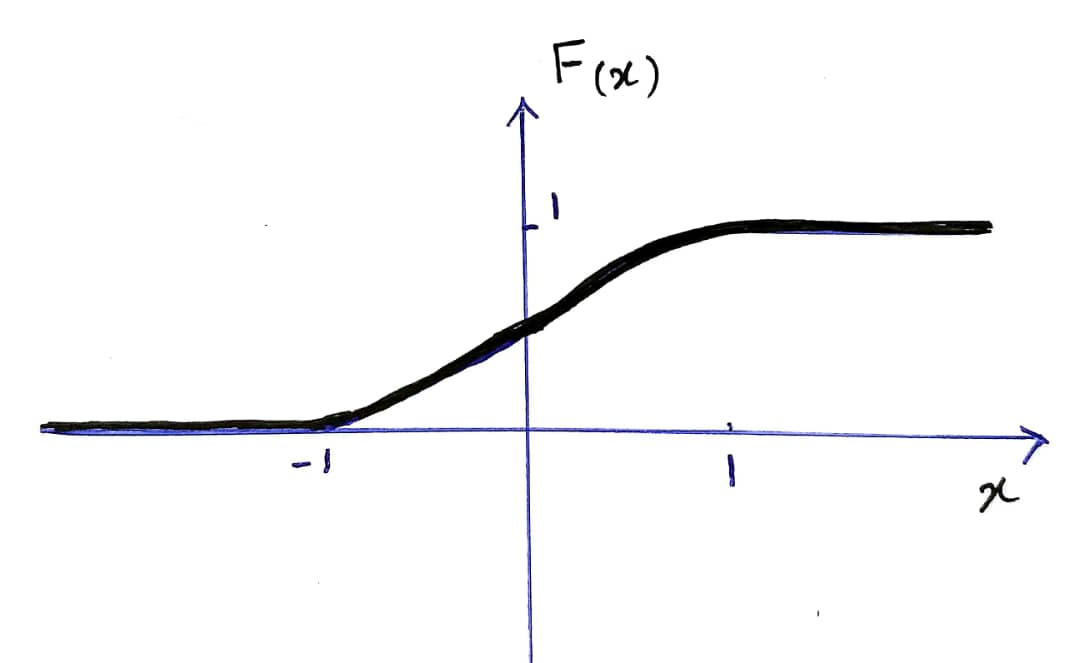
\includegraphics[width=0.6\textwidth]{image002.png}
    \caption{Flux for a beam of particles perpendicular to a surface $A$.\label{fig:flux}}
\end{figure}

\begin{appr}\textbf{Flux}. Consider a beam of particles with velocity $\bm{v}$ and numerical density $n_d = N/V$ (number of particles per unit volume). The number $N_c$ of particles crossing a \textit{flat} area $A$, with unit normal $\bm{\hat{n}} \parallel \bm{v}$, during a time interval $\Delta t$, is given by the total number of particles inside the green region in fig. \ref{fig:flux}, meaning that:
\begin{align}\label{eqn:flux}
    N_c = n_d \cdot \underbrace{\norm{\bm{v}} \Delta t A}_{\mathclap{\text{Volume of the region}}}  \equiv \norm{\bm{J}} \Delta t A
\end{align}   
The quantity $\norm{\bm{J}}$ defined by the relation (\ref{eqn:flux}) is called \textbf{flux}, and represents the number of particles crossing a unit area during a unit time interval. Comparing the left and right hand sides, we obtain the vector relation:
\begin{align*}
    \bm{J} \equiv n_d \bm{v}
\end{align*}
\end{appr}



\begin{exo}[Flux: general case] \label{exo:flux}
    Show that for a generic $\bm{\hat{n}}$ (not necessarily $\parallel \bm{v}$), the number of particles crossing $A$ during the time interval $\Delta t$ is given by:
    \begin{align*}
        N_c = \Delta t A \bm{J}\cdot \bm{\hat{n}}
    \end{align*} 
\end{exo}

The comparison with the equation of state (\ref{eqn:state}) of the ideal gas leads to identify:
    \begin{align}\label{eqn:temperature}
        T = \frac{2}{3} \frac{\mathcal{E}}{n R} \Leftrightarrow \mathcal{E}= \frac{3}{2} n R T   
    \end{align}
This result will be obtained also later when we will derive the equation of state directly from Statistical Mechanics.

\medskip

Substituting (\ref{eqn:temperature}) in (\ref{eqn:rho-p-f}) leads to:
\begin{align*}
    \rho_p(\bm{p}) = (2 \pi m k_B T)^{-3/2} \exp\left(-\frac{\norm{\bm{p}}^2}{2m} \frac{1}{k_B T}  \right)
\end{align*}
where $k_B = R/N_A = \SI{1.3807e-23}{\J\per\K}$ is the Boltzmann constant. 

Equivalently, the velocity distribution is given by:
\begin{align}\label{eqn:velocity-temperature}
    \rho_v(\bm{v}) = \left(\frac{m}{2 \pi k_B T} \right)^{3/2} \exp\left(-\frac{m \norm{\bm{v}}^2}{2k_B T} \right)
\end{align}

\begin{exo}[Speed averages]
    \begin{enumerate}[label=\alph*.]
        \item Use (\ref{eqn:velocity-temperature}) to calculate the average speed, $\langle \norm{\bm{v}} \rangle$, of particles in a gas at temperature $T$. Apply this for $\operatorname{H}_2$, He, $\operatorname{N}_2$, $\operatorname{O}_2$. 
        
        In order to calculate $m$, remember that $N_A \cdot m$ is the molar mass $M_{\mathrm{mol}}$ of the atom (or molecule) of a given gas. So, for example, $M_{\operatorname{O}_2} = 2 \cdot \SI{16}{\g} = \SI{32}{\g}$ is the mass of a mole of $\operatorname{O}_2$, whereas $M_{\operatorname{He}} = \SI{2}{\g}$. 
        \item Determine also $\langle v_\alpha \rangle$, $\langle |v_\alpha| \rangle$, and $\langle \norm{\bm{v}}^2 \rangle$, with $\alpha \in \{x,y,z\}$. Compare $\langle |\bm{v}| \rangle$ with $\sqrt{\langle \norm{\bm{v}}^2 \rangle}$ and notice how they depend on $m$ and $T$.
        \item Determine the mean kinetic energy of a particle of $\operatorname{H}_2$, $\operatorname{He}$, $\operatorname{N}_2$ and O$_2$ at $T=\SI{300}{\K}$.
        \item Determine the number of collisions $n_c$ with a wall per unit time and unit area. Show that:
        \begin{align*}
            n_c = \frac{N}{V} \frac{\langle |v_\alpha| \rangle}{2} = \frac{P}{\sqrt{2 \pi R M_{\mathrm{mol} }T}} N_A   
        \end{align*}
        Show that at atmospheric pressure $P=\SI{1}{atm} = \SI{1.013e5}{\N\per\m\squared}$, $T=\SI{300}{\K}$ for a gas of $\operatorname{O}_2$, we have $n_c= \SI{2.7e23}{\per\s\per\m\squared}$.
    \end{enumerate}
\end{exo}

\begin{exo}
    \textit{Do exercise 3.3 in the textbook}. 
\end{exo}
\end{document}
